\chapter{Desarrollo de la interfaz de usuario}
En Ingeniería del Software nos enseñaron que para añadir una interfaz de usuario a un sistema ya hecho no había que modificar el sistema ya existente. Ese ha sido el principio en el que me he basado para hacer la aplicación web que se usa como interfaz de usuario y que voy a explicar a continuación.

\section{Herramienta usada}
A la hora de hacer una interfaz de usuario en \textit{Python} tenía dos opciones: o bien hacer una interfaz usando \texttt{PyQt} (\url{https://wiki.python.org/moin/PyQt}) o bien hacer una \textit{aplicación web}. Finalmente, me decanté por hacer una aplicación web por las varias razones. En primer lugar, una aplicación web \textit{responsive} puede usarse tanto desde un teléfono móvil como desde un ordenador. Además, el uso de una aplicación web permite que varias personas trabajen a la vez sobre la misma usando una base de datos centralizada, en lugar de tener una copia de los datos en cada ordenador.

Cuando ya decidí qué tipo de interfaz de usuario haría, pasé a pensar con qué \textbf{herramienta} iba a hacerla. Estuve pensando en \texttt{Flask} (\url{http://flask.pocoo.org/}), pero finalmente lo descarté porque es un \textit{framework} que se usa (o se debería de usar) para hacer aplicaciones sencillas. De hecho, su eslogan es \textit{A Python Microframework}. A parte de esto, su documentación es un poco pobre. También estuve pensando en \texttt{Django} (\url{https://www.djangoproject.com/}). \texttt{Django} es fácilmente escalable, con sólo cambiar una línea en un fichero de configuración y hacer algún que otro pequeño ajuste más podemos pasar de usar \texttt{SQLite3} a usar \texttt{PostgreeSQL}, es decir, podemos pasar de usar un gestor de base de datos de ``juguete'' a uno muy potente. Además, tiene una documentación buenísima que incluye un montón de ejemplos ya hechos, además de un montón de explicaciones con muchísimo detalle. Y no solo eso, tiene además una comunidad enorme detrás, por lo que cualquier problema que surja estará resuelto en internet con bastante probabilidad.

\begin{figure}
\centering
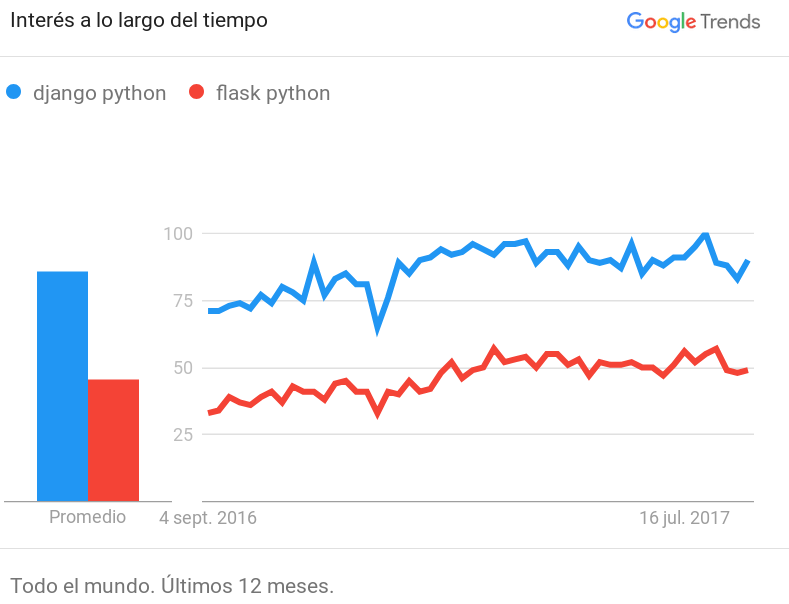
\includegraphics[width=0.7\textwidth]{img/django_flask_trends}
\caption{Interés sobre \texttt{Django} (en azul) y sobre \texttt{Flask} a lo largo del último año en todo el mundo. Datos: Google Trends (\url{https://g.co/trends/CgxUq})}
\label{djangoflasktrends}
\end{figure}

De hecho, si consultamos los datos ofrecidos por \textit{Google Trends} (\hyperref[djangoflasktrends]{Figura \ref*{djangoflasktrends}}) podemos ver que \texttt{Django} es mucho más popular que \texttt{Flask}. Esta es una razón más para elegir uno sobre el otro. ¿Por qué? Porque si un \textit{framework} es popular, significa que tendrá una comunidad que lo mantendrá y dará soporte durante mucho tiempo. 
